\documentclass{VUMIFPSbakalaurinis}
\usepackage{algorithmicx}
\usepackage{algorithm}
\usepackage{algpseudocode}
\usepackage{amsfonts}
\usepackage{amsmath}
\usepackage{bm}
\usepackage{caption}
\usepackage{color}
\usepackage{float}
\usepackage{graphicx}
\usepackage{listings}
\usepackage{subfig}
\usepackage{wrapfig}
\usepackage{tikz}

\usepackage{enumitem}
\setitemize{noitemsep,topsep=0pt,parsep=0pt,partopsep=0pt}
\setenumerate{noitemsep,topsep=0pt,parsep=0pt,partopsep=0pt}

% Ignore all trivial warnings
\hbadness=5000
% Titulinio aprašas
\university{Vilniaus universitetas}
\faculty{Informatikos institutas}
\department{Programų sistemų katedra}
\papertype{Bakalauro baigiamasis darbas }
\title{Srautinio apdorojimo modulių generavimas kintant rodiklių duomenų struktūrai}
\titleineng{Generation of Stream Processing Modules upon Change of Indicator Data Structure}
\author{Vytautas Žilinas}
\supervisor{lekt. Andrius Adamonis}
\reviewer{assoc. prof., dr. Karolis Petrauskas}
\date{Vilnius – \the\year}

% Nustatymai
% \setmainfont{Palemonas}   % Pakeisti teksto šriftą į Palemonas (turi būti įdiegtas sistemoje)
\bibliography{bibliografija}

\begin{document} 
\maketitle

\cleardoublepage\pagenumbering{arabic}
\setcounter{page}{2}

\sectionnonumnocontent{Santrauka}
Šį darbą sudaro teorinė ir eksperimentinė dalis. Teorinėje dalyje apibrėžiamas rodiklis, jo struktūra ir struktūros pokyčiai. Apibrėžiami kokie yra įmanomi pokyčiai ir kaip eksperimentinėje dalyje kuriamas sprendimas prie pokyčių prisitaikys. Specifikuojama duomenų struktūra ir duomenų struktūrų apjungimo ir skirtumo operacijas. Apibrėžiamas srautinis apdorojimas ir pasirenkama sistema, kuri bus naudojama eksperimentinėje dalyje. Remiantis gautais rezultatais
nustatoma, kad šiam uždaviniui spręsti pasirenkama "Heron" srautinio apdorojimo sistema. Remiantis pasirinkta srautinio apdorojimo sistema ir apibrėžta rodiklių duomenų struktūra, eksperimentui nusprendžiama generuoti srautinio apdorojimo modulius parašytus "Python" programavimo kalba. Eksperimentinėje dalyje remiantis pasiūlytu modeliu realizuojama bandomoji sistemos versija. Atliekant skirtingų kiekių rodiklių duomenų ir rodiklių duomenų pokyčių simuliaciją stebėjimais analizuojamas šios sistemos tinkamumas apibrėžtam uždaviniui spręsti. Gauti tyrimų rezultatai lyginami, pateikiamos išvados. Taip įrodoma, kad toks sprendimas gali būti įgyvendinamas ir kad kodo generavimas ir srautinio apdorojimo sistema "Heron" yra tinkamas sprendimas kintančių rodiklių uždaviniui spręsti.
\raktiniaizodziai{srautinis apdorojimas, kodo generavimas, rodikli, rodiklio duomens pokyčiai}   

\sectionnonumnocontent{Summary}
This work consists of a theoretical and an experimental part. Theoretical part defines the indicator, its structure and changes in indicator structure. It define what changes are possible and how the developed solution in the experimental part will adapt to the changes, specifies the data structure and data structure merging and difference operations, defines stream processing and selects the system to be used in the experimental part. Based on the results
it is determined that "Heron" stream processing system is chosen to solve this task. Based on the selected stream processing system and the defined data structure of indicator, it is decided to generate streaming modules written in "Python" programing language. In the experimental part, a pilot version of the system is implemented based on the proposed model. By doing the simulation using varying amounts of indicators and indicator changed, the suitability of this system for a defined task is tested. The results of this research are compared and conclusions are given. This demonstrates that such a solution can be implemented and that the code generation and streaming system "Heron" is the right solution to deal with the challenge of changing indicators.
\keywords{stream processing, code generation, indicator, indactor structure change}

\tableofcontents

\sectionnonum{Įvadas}
 
% TODO: Įžangoje apžvelgti srautinį apdorojimą ir kodo generavimą.
Šiame darbe yra nagrinėjamas rodiklių duomenų apdorojimas ir kuriamas sprendimas galintis prisitaikyti prie kintančių rodiklių duomenų struktūros. Rodiklių duomenimis vadiname duomenis, aprašančius kažkokių objektų savybes arba veiklos procesų rezultatus. Šiuos duomenis galima transformuoti, analizuoti ir grupuoti pagal pasirinktus rodiklius, pavyzdžiui: bazinė mėnesinė alga, mirusiųjų skaičius pagal mirties priežastis, krituliai per metus. Taip pat rodiklių struktūra gali keistis laikui bėgant: objektų atributų taksonomija (pvz. mirties priežasčių sąrašas, finansinių sąskaitų sąrašas) arba įrašo atributų sąrašai. Surenkamu rodiklių duomenų kiekis visada didėja, taip pat ir duomenų kiekis, kuriuos reikia apdoroti pagal rodiklius auga, todėl standartiniai sprendimai, pavyzdžiui reliacinės duomenų bazės netinka dėl ilgos apdorojimo trukmės. Rodiklių duomenų bazės pasižymi tuo, kad duomenys į jas patenka iš daug skirtingų tiekėjų ir patekimo laikas tarp tiekėjų nėra sinchronizuojamas, o suagreguotą informaciją vartotojai gali užklausti bet kurio metu. Todėl šiame darbe bus nagrinėjamas srautinis duomenų apdorojimas, kuris patenkančius duomenis apdoros realiu laiku, ir saugos jau apdorotus.  \par
Realaus laiko duomenų apdorojimas (angl. Real-time data processing) yra jau senai nagrinėjamas, kaip būdas apdoroti didelių kiekių duomenis (angl. Big data). Vienas iš realaus laiko apdorojimo sprendimų yra srautinis duomenų apdorojimas \cite{BigData, StreamProcessingInData}. Srautinis duomenų apdorojimas (angl. stream processing) – programavimo paradigma, kuri yra ekvivalenti duomenų srauto programavimo (angl. dataflow programming) paradigmai \cite{shortstreamproc}. 
Duomenų tėkmės programavimo paradigmos idėja yra, kad programa susidaro iš skirtingu modulių, kurie nepriklauso vienas nuo kito, ir tai leidžia sukonstruoti paraleliai skaičiuojančias programas. 
Vienas iš pirmųjų duomenų tėkmės programavimo kompiliatorių yra BLODI - blokų diagramų kompiliatorius (angl. BLOck DIagram compiler), su kuriuo buvo kompiliuojamos BLODI programavimo kalba parašytos programos \cite{kelly1961block}.  Šia kalba parašytos programos atitinka inžinerinę elektros grandinės schemą, kur duomenys keliauja per komponentus kaip ir elektros grandinėje. Pasinaudojant šiai programavimo paradigmai sukurtai sistemai bus sukurtas sprendimas, kuris generuos modelius, kurie galės apdoroti rodiklių duomenis ir talpins jau apdorotus duomenis kitoje talpykloje \cite{8Requirements}. 
\par
Kadangi rodiklių yra daug skirtingų ir jie laikui bėgant gali kisti reikia, kad sprendimas kuris juos apdoros galės prisitaikyti prie poreikiu. Yra keli būdai kaip tai galima išspręsti:
\begin{itemize}
    \item Rankinio atnaujinimo sprendimas. Sukuriamas sprendimas pagal esamus reikalavimus ir išskiriamas žmogus, kuris pagal naujus poreikius gali sukurti naujas arba pakeisti esamas apdorojimo programas. 
    \item Universalus sprendimas. Sukuriamas srautinio duomenų apdorojimo sprendimas, kuris apdoroja visus duomenis pagal visus įmanomus rodiklius.
    \item Kodo generavimo sprendimas. Sukuriamas sprendimas, kuris generuoja srautinio duomenų apdorojimo programas pagal iš anksto aprašytą struktūrą.  
\end{itemize}   
Šie sprendimai turi būti pritaikyti pagal sprendžiama problemą. Jei nėra numatomas kitimas pagal ką turi būti apdorojami duomenis, tai galima pasirinkti ir rankinio apdorojimo sprendimą, kadangi nėra didelės tikimybės, kad teks keisti sprendimą. Toks sprendimas tiktų apdorojant išmaniųjų skaitiklių duomenis \cite{skaitikliai}. Universalus sprendimas taip pat gali būti tinkamas jei įeinantis duomenis yra specifiški ir yra poreikis juos visus apdoroti. Toks sprendimas gali būti aktualus apdorojant duomenis iš sensorių, kurie matuoja namų būsena (temperatūra, drėgmę ir t.t.) ir bet koks naujas sensorius taip pat turi būti prijungtas ir apdorotas \cite{yang2017iot}. Šiame darbe buvo pasirinkta naudoti kodo generavimą siekiant sukurti sprendimą tinkanti bendram atvejui, kai duomenis yra nekonkretus ir ne visi reikalingi ir rodikliai kinta dažnai siekiant išgauti kuo daugiau informacijos iš įeinančių duomenų. \par
Kodo generavimas - todo \par
Darbe bus nagrinėjamas sprendimas generuojantis srautinio apdorojimo modulius pagal ateinančius rodiklių duomenis. 
Kadangi rodikliai yra  
Šiame darbe kuriamas sprendimas yra aktualus, kai kinta duomenų struktūra ir norėtume šis sprendimas prisitaiko 
prie duomenų pokyčių kurdamas naujus apdorojimo modulius.


Tikslas: Sukurti rodiklių duomenų srautinio apdorojimo platformos architektūrą, kuri, naudojant kodo generavimą, dinamiškai prisitaiko prie rodiklių duomenų struktūrų pokyčių.

Uždaviniai:
\begin{enumerate}
    \item Apibrėžti rodiklių duomenų modelį ir galimus rodiklių duomenų struktūros pokyčius.
    \item Apibrėžti, kaip specifikuoti duomenų struktūrą ir duomenų struktūrų versijų specifikacijų apjungimo ir skirtumo operacijas.
    \item Atlikus šaltinių analizę pasirinkti srautinio duomenų apdorojimo sistemą, joje sukurti sudarytos architektūros sprendimą ir atlikti bandymus.
\end{enumerate}

\section{Rodiklių duomenys}

Rodiklių duomenys - tai duomenis, kurie apibrėžia bet kokius duomenis, kuriuos galime grupuoti pagal tam kitus elementus. Rodiklį sudaro pirminis raktas, kuris susideda iš vieno arba daug duomenų ir reikšmių sąrašas, kurį galime grupuoti pagal apibrėžtą raktą.      
Rodiklių duomenų gali būti daug todėl reikia bendro modelio, kuris gali apibrėžti visus įmanomus rodiklius. 
\subsection{Rodiklių duomenų modelis}

Darbo tikslui išpildyti buvo sukurtas modelis, kurio pagalba galime apibrėžti rodiklį. Pagal šį apibrėžimą bus generuojama srautinio apdorojimo architektūra.

\begin{figure}[H]
    \centering
    \includegraphics[width=1\textwidth]{img/rodiklis.jpg}
    \caption{Rodiklis}
    \label{img:rodiklis}
\end{figure}

Šiame darbe šis rodiklis bus užrašomas skaidant į dvi dalis: \\
Raktas ir apribojimai:
\[ [\text{Raktas 1, Raktas N}]
    \>\> ; \>\>  
    \begin{array}{|c|c|}
        \hline
        \text{Apribojimas 1} & \text{Apribojimas N} \\ 
        \hline
        \text{Reikšmė 1} & \text{Reikšmė N} \\ 
        \text{Operatorius 1} & \text{Operatorius N} \\
        \text{Riba 1} & \text{Riba N} \\
        \hline 
   \end{array}
\]
Reikšmės: \\
\[
    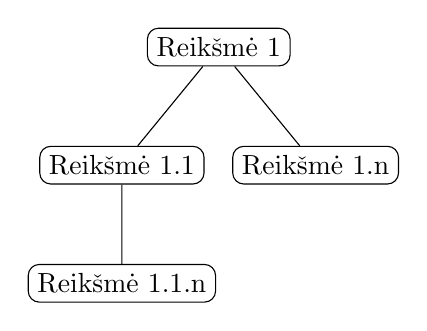
\begin{tikzpicture}[sibling distance=7em,
        every node/.style = {shape=rectangle, rounded corners,
                             draw, align=center,
                             top color=white, bottom color=white}]
        \node {Reikšmė 1}
                child { node {Reikšmė 1.1} 
                    child { node { Reikšmė 1.1.n} } }
                child { node {Reikšmė 1.n} } ;
    \end{tikzpicture} 
    \>\>\>\>\>\>\>\>
    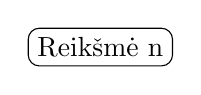
\begin{tikzpicture}[sibling distance=10em,
        every node/.style = {shape=rectangle, rounded corners,
            draw, align=center,
            top color=white, bottom color=white}]]
        \node {Reikšmė n} ;
    \end{tikzpicture}  
\]
\section{Rodiklių duomenų pokyčiai}

Kadangi einant laiku duomenis gali keistis ir atitinkamai gali keistis ir rodiklių duomenų tipas, kuriuos reikia surinkti. Tarkime mes turime rodiklį, kuris apibrėžia žmogaus, kuris dirba pagal terminuotą darbo sutartį, metines pajamas, kurios susideda iš gaunamo atlyginimo ir premijų:
Raktas ir apribojimai:
\[ [\text{Žmogus, Metai}]
    \>\> ; \>\>  
    \begin{array}{|c|}
        \hline
        \text{Terminuotą darbo sutartis}  \\ 
        \hline
        \text{Darbo sutarties tipas} \\ 
        \text{LYGU}  \\
        \text{TERMINUOTA} \\
        \hline 
   \end{array}
\]
Reikšmės: \\
\[
    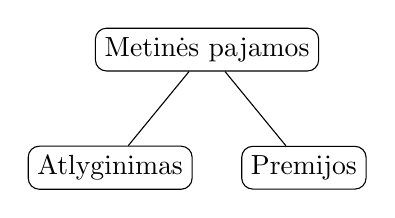
\begin{tikzpicture}[sibling distance=7em,
        every node/.style = {shape=rectangle, rounded corners,
                             draw, align=center,
                             top color=white, bottom color=white}]
        \node {Metinės pajamos}
                child { node {Atlyginimas} }
                child { node {Premijos} } ;
    \end{tikzpicture} 
\]
Pavyzdžiui, jei atsiranda poreikis fiksuoti, ne tik iš gaunama atlygimą ir premiją, bet ir iš loterijose laimėtus pinigus. Taip pat tarkime, jog terminuota darbo sutartis buvo išskaidyta į terminuotą darbo sutartį ir laikinojo darbo sutartį ir mums reikia įtraukti duomenis pagal abu apribojimus. Mūsų rodiklis, turėtų atsinaujinti atitinkamai:

Raktas ir apribojimai:
\[ [\text{Žmogus, Metai}]
    \>\> ; \>\>  
    \begin{array}{|c|c|}
        \hline
        \text{Terminuotą darbo sutartis} & \text{Laikinojo darbo sutartis} \\ 
        \hline
        \text{Darbo sutarties tipas} & \text{Darbo sutarties tipas} \\ 
        \text{LYGU} & \text{LYGU} \\
        \text{TERMINUOTA} & \text{LAIKINOJI} \\
        \hline 
   \end{array}
\]
Reikšmės: \\
\[
    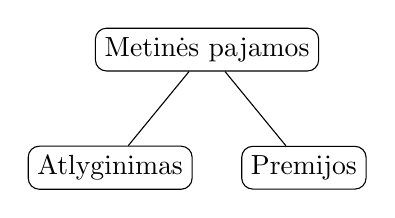
\begin{tikzpicture}[sibling distance=7em,
        every node/.style = {shape=rectangle, rounded corners,
                             draw, align=center,
                             top color=white, bottom color=white}]
        \node {Metinės pajamos}
            child { node {Atlyginimas} }
            child { node {Premijos} } ;
    \end{tikzpicture} 
    \>\>\>\>\>\>\>\>
    \begin{tikzpicture}[sibling distance=10em,
        every node/.style = {shape=rectangle, rounded corners,
            draw, align=center,
            top color=white, bottom color=white}]]
        \node {Loterijų laimėjimai} ;
    \end{tikzpicture}  
\]

\subsection{Galimi pokyčiai}

\subsubsection{Pirminis raktas}
Mes savo rodiklyje pakeitėme apribojimus ir reikšmes, tačiau nekeitėme pirminio rakto todėl, kad tokiu atveju grupavimas nebeturėtų prasmės. Tarkime, kad norime nuo 2019 metų rinkti duomenis ne metinius, o kas mėnesį. Tokiu atveju jau surinkti duomenis nebeturi prasmės, nes bandoma lyginti metinius rezultatus su mėnesiais. Jei tai toks elementas, kuris gali kisti ir nėra renkama reikšmė tai turėtų būti apibrėžiama kaip apribojimas. Jei yra poreikis keisti pirminį raktą, reikia kurti naują rodiklį ir, jei yra poreikis pagal jį suagreguoti naujus ir istorinius duomenis, turi būti iš naujo apdoroti visi turimi duomenys.     

\subsubsection{Apribojimai}

\subsubsection{Reikšmės}


\section{Medžiagos darbo tema dėstymo skyriai}
Medžiagos darbo tema dėstymo skyriuose išsamiai pateikiamos nagrinėjamos temos
detalės: pradiniai duomenys, jų analizės ir apdorojimo metodai, sprendimų
įgyvendinimas, gautų rezultatų apibendrinimas.

Medžiaga turi būti dėstoma aiškiai, pateikiant argumentus. Tekste dėstomas
trečiuoju asmeniu, t.y. rašoma ne „aš manau“, bet „autorius mano“, „autoriaus
nuomone“. Reikėtų vengti informacijos nesuteikiančių frazių, pvz., „...kaip jau
buvo minėta...“, „...kaip visiems žinoma...“ ir pan., vengti grožinės
literatūros ar publicistinio stiliaus, gausių metaforų ar panašių meninės
išraiškos priemonių.

Skyriai gali turėti poskyrius ir smulkesnes sudėtines dalis, kaip punktus ir
papunkčius.

\sectionnonum{Rezultatai}

\begin{enumerate}
    \item Apibrėžta rodiklių duomenų struktūra ir galimi duomenų struktūros pokyčiai.
    \item Pasirinktai srautinio duomenų apdorojimo sistemai sukurto sprendimo atliktų eksperimentų rezultatai - generuojamas kodas ir jo savybes. 
\end{enumerate}

\sectionnonum{Išvados}
Rezultatų ir išvadų dalyje išdėstomi pagrindiniai darbo rezultatai (kažkas
išanalizuota, kažkas sukurta, kažkas įdiegta), toliau pateikiamos išvados
(daromi nagrinėtų problemų sprendimo metodų palyginimai, siūlomos
rekomendacijos, akcentuojamos naujovės). Rezultatai ir išvados pateikiami
sunumeruotų (gali būti hierarchiniai) sąrašų pavidalu. Darbo rezultatai turi
atitikti darbo tikslą.

\printbibliography[heading=bibintoc] 


\appendix 


\end{document}
